\section{Executed results}
\label{sec:results}

This section distinguishes populated archived outputs from three corrected Phase~6 executions. Each corrected output has a new result identifier, parent link, versioned sidecar, and artifact hashes. Historical values remain unchanged; interpretation follows Section~\ref{sec:experimental-design}.

\subsection{Single-sequence posterior summaries}
Figure~\ref{fig:gaussian-result-paper} shows a Gaussian sequence with two true changepoints. The boundary-event posterior concentrates near the generating changes while retaining a smaller shoulder of ambiguity before the first jump. The joint-MAP signal reflects this local uncertainty by inserting a short intermediate segment. Table~\ref{tab:gaussian-summary-paper} shows that the selected and modal segment count is four while the posterior mean is $4.742$, illustrating why an exported partition and posterior uncertainty over $k$ should not be collapsed into one object.

\begin{figure*}[t]
  \centering
  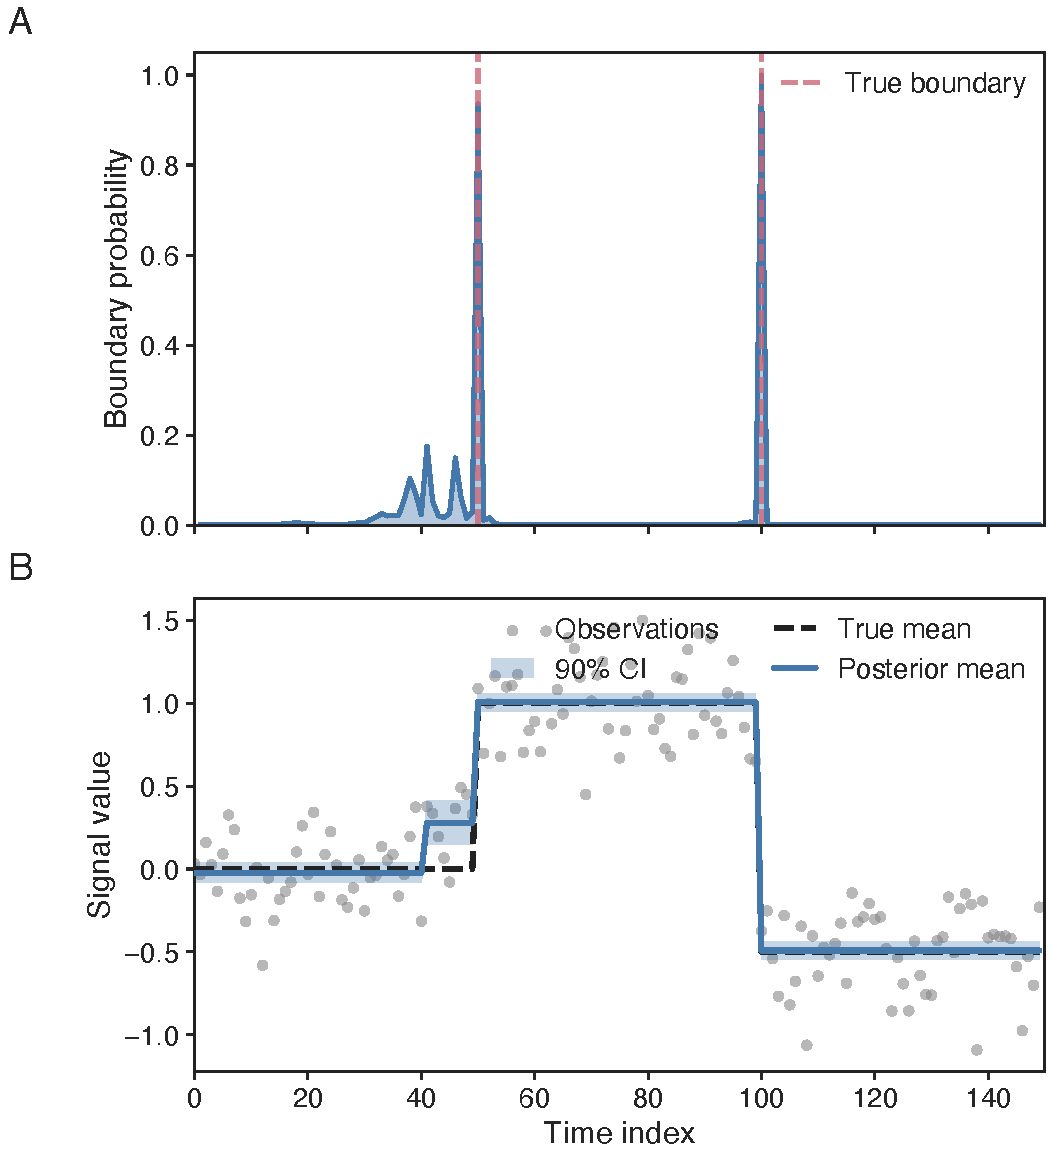
\includegraphics[width=0.94\textwidth]{shared/figures/results/fig1_synthetic_gaussian.pdf}
  \caption{Executed Gaussian illustration. Top: marginal boundary-event posterior with generating changepoints shown by dashed lines. Bottom: observations, latent signal, joint-MAP segmentation, and 90\% segment-level posterior intervals.}
  \label{fig:gaussian-result-paper}
\end{figure*}

\begin{table}[t]
\centering
\small
\begin{tabular}{lr}\toprule
Quantity & Value\\\midrule
Selected $k$ (\texttt{k\_ml\_}) & 4\\
Posterior mean $\mathbb{E}[k]$ & 4.742\\
MAP $k$ & 4\\
$\log p(y)$ & -18.031\\
\bottomrule\end{tabular}

\caption{Executed posterior summary for Figure~\ref{fig:gaussian-result-paper}.}
\label{tab:gaussian-summary-paper}
\end{table}

\subsection{Portability across local observation models}
The same global inference code was applied to Gaussian, Poisson, Binomial, and Beta-valued responses (Figure~\ref{fig:family-result-paper}). Table~\ref{tab:family-result-paper} reports the archived synthetic metrics. Gaussian, Binomial, and Beta-valued settings selected the generating three segments; Poisson selected four and had the weakest boundary score and largest reconstruction error in this small benchmark. The result supports interface portability and exposes relative difficulty in the bundled settings; it is not a population-level ranking of families.

\begin{figure*}[t]
  \centering
  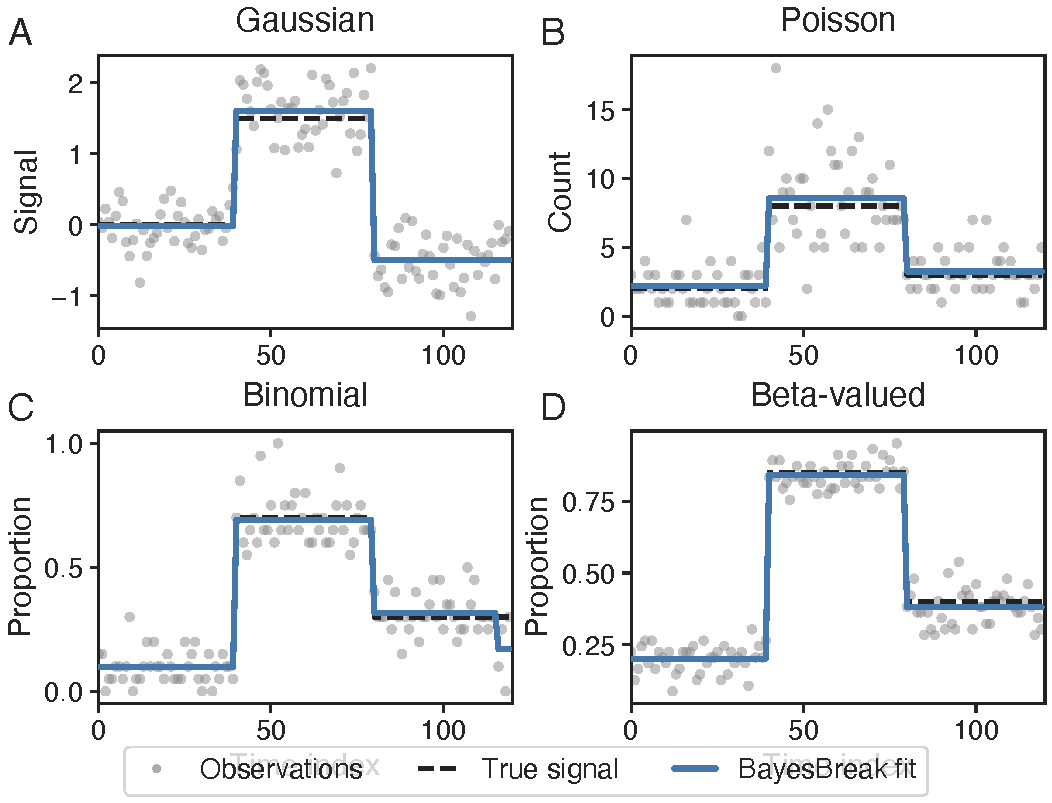
\includegraphics[width=0.95\textwidth]{shared/figures/results/fig2_family_showcase.pdf}
  \caption{Executed family showcase. Gaussian, Poisson, and Binomial use closed-form local conjugate integration; the Beta-valued response uses deterministic one-dimensional quadrature.}
  \label{fig:family-result-paper}
\end{figure*}

\begin{table*}[t]
\centering
\small
\resizebox{0.88\textwidth}{!}{\begin{tabular}{lrrrrrrr}\toprule
Family & n & $k^\star$ & $\hat{k}$ & F1@$\tau$ & MAE & MSE & $-\log p(y)/n$\\\midrule
Gaussian & 120 & 3 & 3 & 0.968 & 0.00 & 0.0023 & 0.191\\
Poisson & 120 & 3 & 4 & 0.777 & 0.20 & 0.4501 & 2.162\\
Binomial & 120 & 3 & 3 & 0.960 & 0.06 & 0.0004 & 2.108\\
Beta-valued & 120 & 3 & 3 & 1.000 & 0.00 & 0.0001 & 2.620\\
\bottomrule\end{tabular}
}
\caption{Executed synthetic summary across local observation models. The Beta-valued row is quadrature-based rather than closed-form conjugate.}
\label{tab:family-result-paper}
\end{table*}

\subsection{Calibration and latent-group segmentation}
Repeated Gaussian simulations produced a reliability curve close to the diagonal, with archived ECE approximately $0.010$ and Brier score approximately $0.011$ (Figure~\ref{fig:calibration-template-paper}a). These values support calibration in the generating design, not robustness to arbitrary misspecification.

The latent-group experiment used 24 sequences of length 80 from two known synthetic groups at noise standard deviation $1.0$. It achieved 96\% hard assignment accuracy, with one misassignment and visible ambiguity around the class boundary (Figure~\ref{fig:calibration-template-paper}b). Group-specific boundary marginals concentrate near the generating templates. The result is evidence for the finite score-clustering objective in Equation~\eqref{eq:latent-group-objective}; it is not evidence for normalized-mixture identifiability.

\begin{figure*}[t]
\centering
\begin{subfigure}[t]{0.42\textwidth}
  \centering
  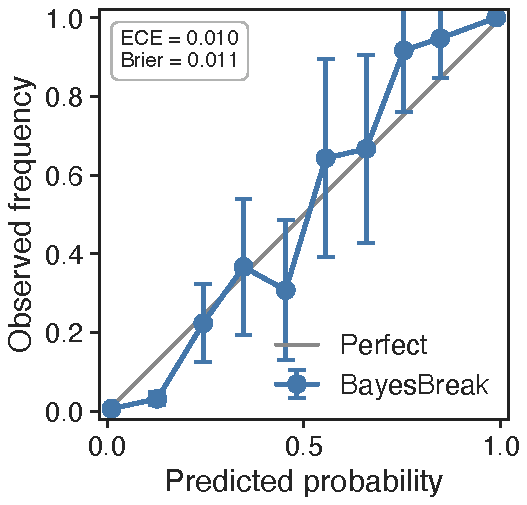
\includegraphics[width=\linewidth]{shared/figures/results/fig3_boundary_calibration.pdf}
  \caption{Boundary-event reliability.}
\end{subfigure}\hfill
\begin{subfigure}[t]{0.54\textwidth}
  \centering
  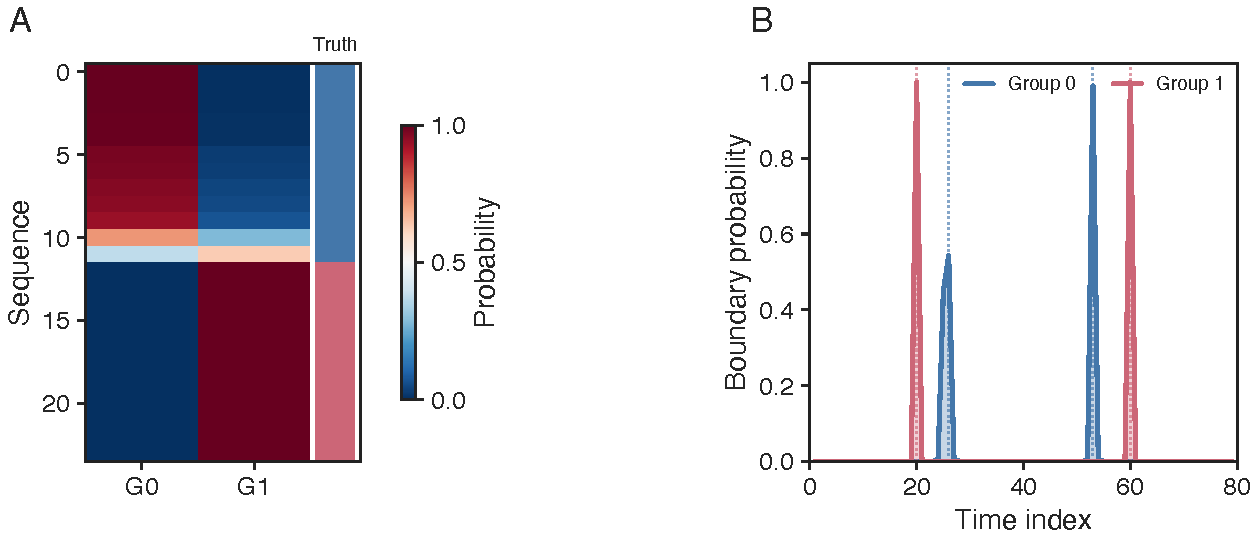
\includegraphics[width=\linewidth]{shared/figures/results/fig4_latent_groups_cropped.pdf}
  \caption{Latent-group assignments and group-specific boundary marginals.}
\end{subfigure}
\caption{Executed uncertainty and template diagnostics. Panel (a) reports ECE $\approx0.010$ and Brier $\approx0.011$ in the archived Gaussian calibration experiment. Panel (b) reports 96\% hard recovery for the declared two-template synthetic setting.}
\label{fig:calibration-template-paper}
\end{figure*}

The corrected stress execution \resultid{RES-BB-SYN-005} evaluated 400 seeded datasets across eight predeclared cells. In the archived-design cell, mean label-invariant hard accuracy was $0.9742$ (95\% interval $0.9536$--$0.9948$) and mean adjusted Rand index was $0.9183$. All 400 objective traces were monotone, every returned final objective equaled the final trace value, and all 1,200 restarts were valid. Recovery degraded under low separation, duplicate templates, higher noise, and shorter sequences, as summarized in Figure~\ref{fig:latent-stress-corrected-paper}. These results support the finite score-clustering criterion in the declared simulations, not normalized-mixture identifiability.

\begin{figure*}[t]
  \centering
  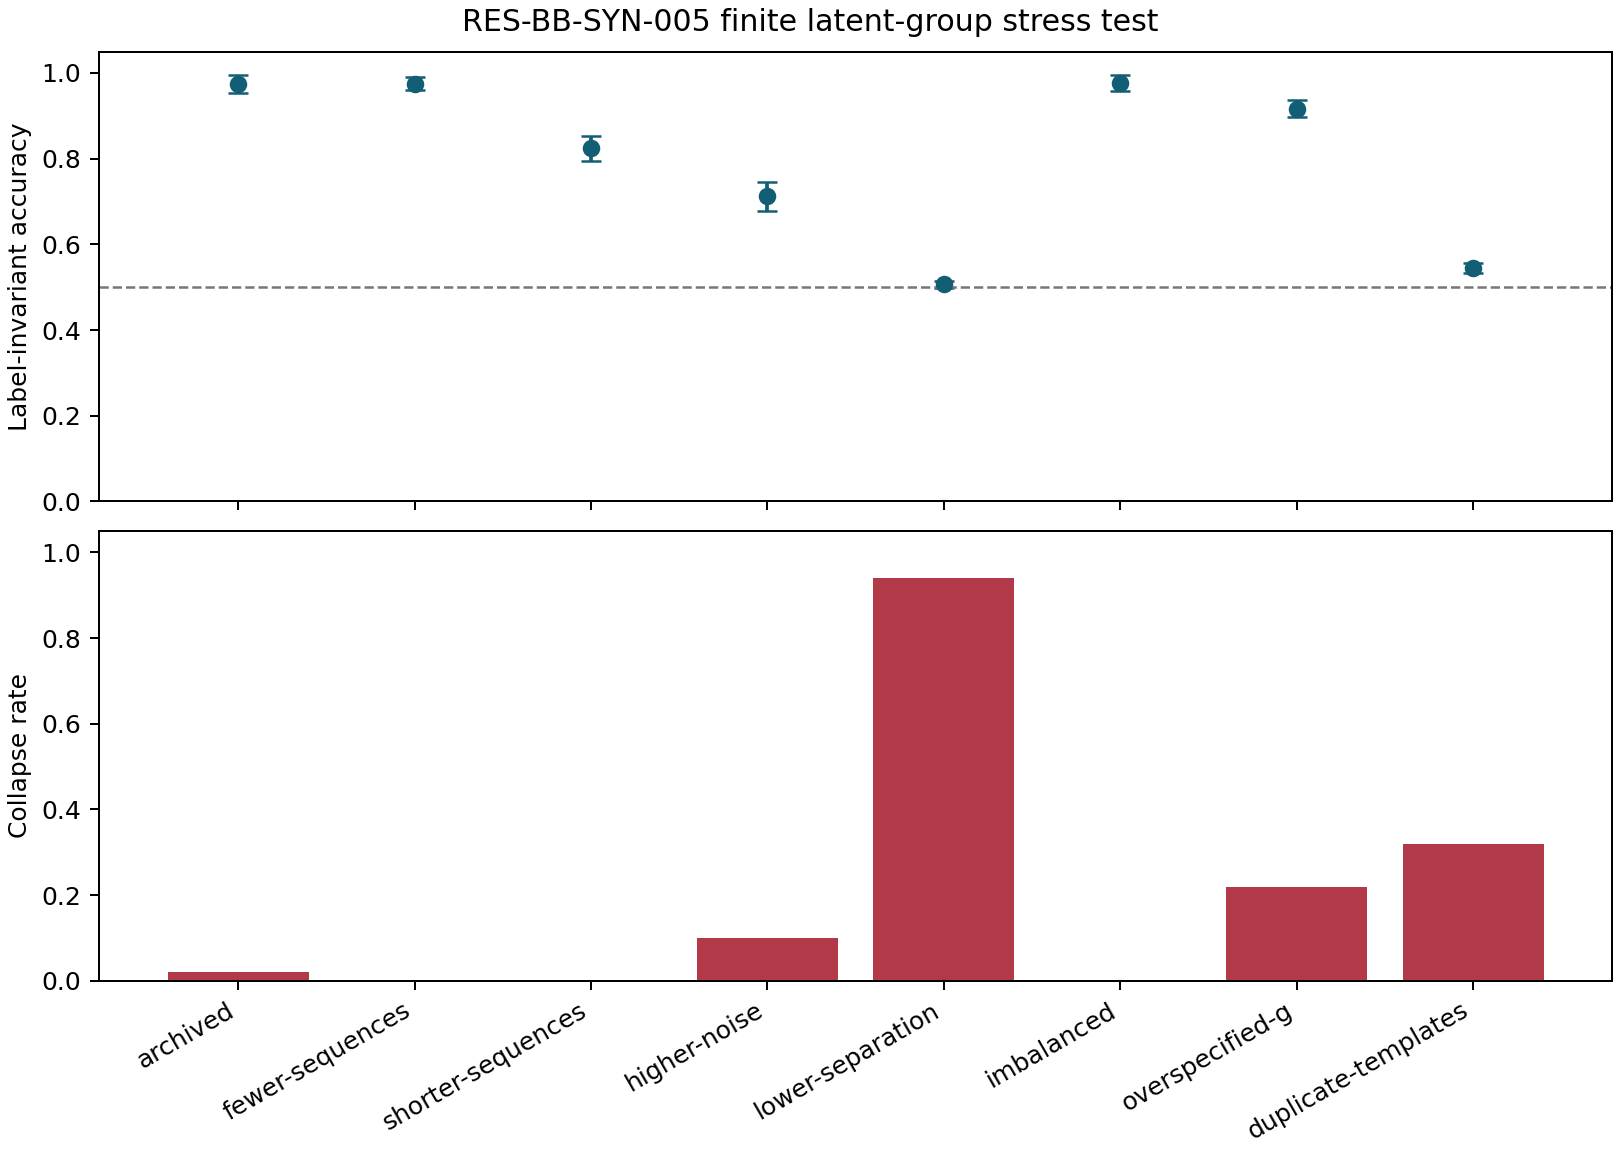
\includegraphics[width=0.88\textwidth]{shared/figures/results/fig_phase6_latent_stress.png}
  \caption{Corrected latent-group stress execution \resultid{RES-BB-SYN-005}. Top: label-invariant hard accuracy with dataset-level 95\% intervals. Bottom: collapsed or duplicate-template rate. The dashed $0.5$ line is a descriptive reference, not a universal recovery threshold.}
  \label{fig:latent-stress-corrected-paper}
\end{figure*}

\subsection{Nonconjugate block approximations}
Table~\ref{tab:nonconjugate-result-paper} compares five local routines in the archived Bernoulli/logistic example, using quadrature as the local reference. Laplace was the fastest listed routine at $0.049$ seconds, whereas quadrature required $0.093$ seconds. Maximum absolute block-score discrepancies were $1.235$ for Laplace, $1.265$ for Jaakkola--Jordan and P\'olya--Gamma mean field, and $14.502$ for expectation propagation. Boundary $F_1$ did not vary monotonically with block-score discrepancy: quadrature and Laplace selected six segments with $F_1=0.286$, whereas three other routines reported $F_1=0.500$ under different selected segment counts.

\begin{table*}[t]
\centering
\scriptsize
\resizebox{0.97\textwidth}{!}{\begin{tabular}{lrrrrrr}\toprule
Method & $\max|\Delta \log A^0|$ & $q_{95}|\Delta \log A^0|$ & median $|\Delta \log A^0|$ & time (s) & F1@$\tau$ & $\hat{k}$\\\midrule
quadrature & 0.000 & 0.000 & 0.000 & 0.093 & 0.286 & 6\\
laplace & 1.235 & 1.188 & 0.980 & 0.049 & 0.286 & 6\\
jj & 1.265 & 1.216 & 1.002 & 0.071 & 0.500 & 3\\
ep & 14.502 & 14.141 & 12.680 & 0.059 & 0.500 & 7\\
pg-vb & 1.265 & 1.216 & 1.002 & 0.072 & 0.500 & 3\\
\bottomrule\end{tabular}
}
\caption{Executed local-approximation trade-off. The observed maximum errors are too large to treat this example as verification of a small uniform segmentwise error bound.}
\label{tab:nonconjugate-result-paper}
\end{table*}

This result demonstrates why segmentation output alone cannot certify a block approximation. The global dynamic program aggregates many local score differences, and a boundary metric can improve despite a worse local approximation. Claim-supporting use of Theorem~\ref{thm:stability-paper} therefore requires a uniform error bound over all admissible segments rather than retrospective agreement in the estimated segmentation.

\subsection{Finite-range runtime behavior}
Figure~\ref{fig:runtime-result-paper} reports length and segment-budget sweeps. At $k_{\max}=20$, mean runtime rose from $0.0455$ seconds at $n=50$ to $1.0585$ seconds at $n=800$ (Table~\ref{tab:runtime-result-paper}). Fitted log--log slopes were approximately $1.07$ in $n$ for $k_{\max}=10$, $1.14$ for $k_{\max}=20$, and $0.88$ in $k_{\max}$ at fixed $n=200$. They summarize this implementation over the measured range; they do not replace the $\Theta(k_{\max}n^2)$ worst-case accounting in Proposition~\ref{prop:complexity-paper}.

\begin{figure*}[t]
  \centering
  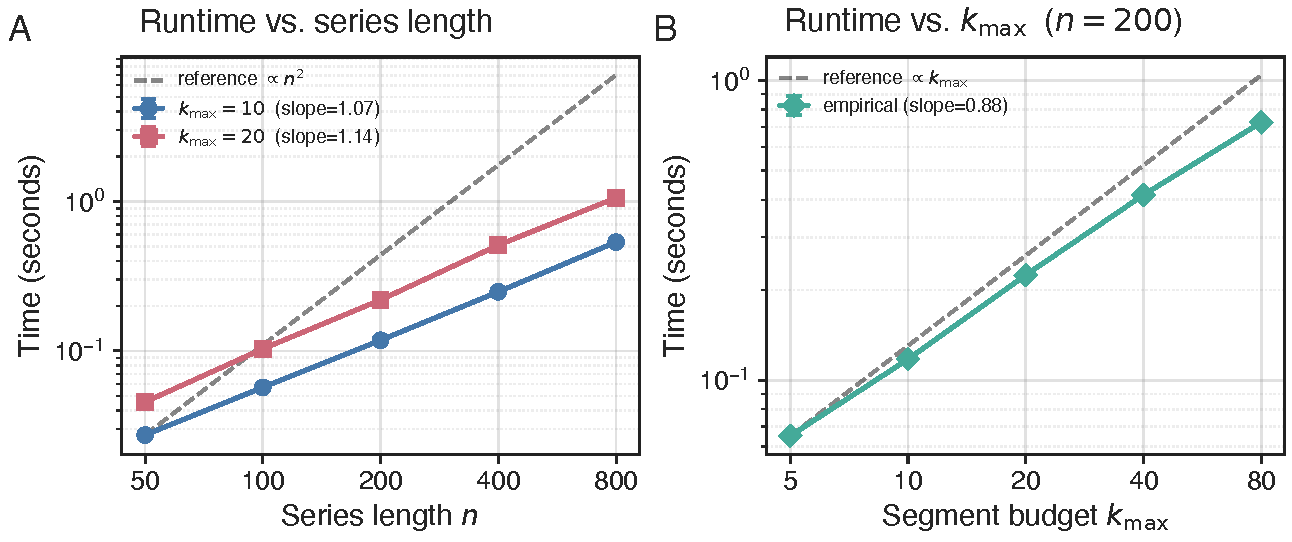
\includegraphics[width=0.92\textwidth]{shared/figures/results/fig5_runtime_scaling.pdf}
  \caption{Executed Gaussian runtime study. Points are means over five repetitions and error bars are one standard deviation. Dashed references show quadratic-in-$n$ and linear-in-$k_{\max}$ guides, not fitted complexity claims.}
  \label{fig:runtime-result-paper}
\end{figure*}

\begin{table}[t]
\centering
\small
\begin{tabular}{rrrr}\toprule
n & $k_{\max}$ & mean (s) & std (s)\\\midrule
50 & 20 & 0.0455 & 0.0008\\
100 & 20 & 0.1033 & 0.0011\\
200 & 20 & 0.2195 & 0.0011\\
400 & 20 & 0.5106 & 0.0307\\
800 & 20 & 1.0585 & 0.0345\\
\bottomrule\end{tabular}

\caption{Archived $k_{\max}=20$ runtime values from the length sweep.}
\label{tab:runtime-result-paper}
\end{table}

\subsection{Four real-data fits}
Table~\ref{tab:real-summary-paper} summarizes the executed case studies. Each fit passed all four archived dynamic-programming checks. Their figures provide fitted segmentation, boundary uncertainty, segment-count posterior information, and in-sample diagnostics. No independent boundary labels were present, so the case studies establish execution and descriptive posterior behavior rather than external accuracy.

\begin{table}[t]
\centering
\small
\caption{Executed real-data fits. The log evidences belong to different data models and are not compared across rows.}
\label{tab:real-summary-paper}
\begin{tabularx}{\columnwidth}{@{}Y C{0.19\columnwidth} C{0.12\columnwidth} C{0.28\columnwidth}@{}}
\toprule
Case & $n$ or shape & $\widehat k$ & Log evidence \\
\midrule
Well-log & 507 & 23 & $-4989.2835$ \\
Array-CGH & $43\times2215$ & 15 & $76359.7996$ \\
S\&P 500 & 566 & 29 & $-1296.6537$ \\
Methylation & 1904 & 15 & $-9518.6675$ \\
\bottomrule
\end{tabularx}
\end{table}

\paragraph{Well-log.}
The archived source contains 4,050 NMR response values and an executed downsampled sequence of $n=507$. Under the index-uniform prior, the Gaussian fit selected 23 segments with log evidence $-4989.283473023698$ (Figure~\ref{fig:welllog-paper}). A separately executed length-cohesion configuration selected 25 segments with log evidence $-4997.147814570523$. These are distinct prior models; the values do not establish a universal preference between index and physical-length priors. Archived comparator scores at tolerance three are agreement with the \BayesBreak MAP boundary set, not verified geology.

\begin{figure*}[t]
  \centering
  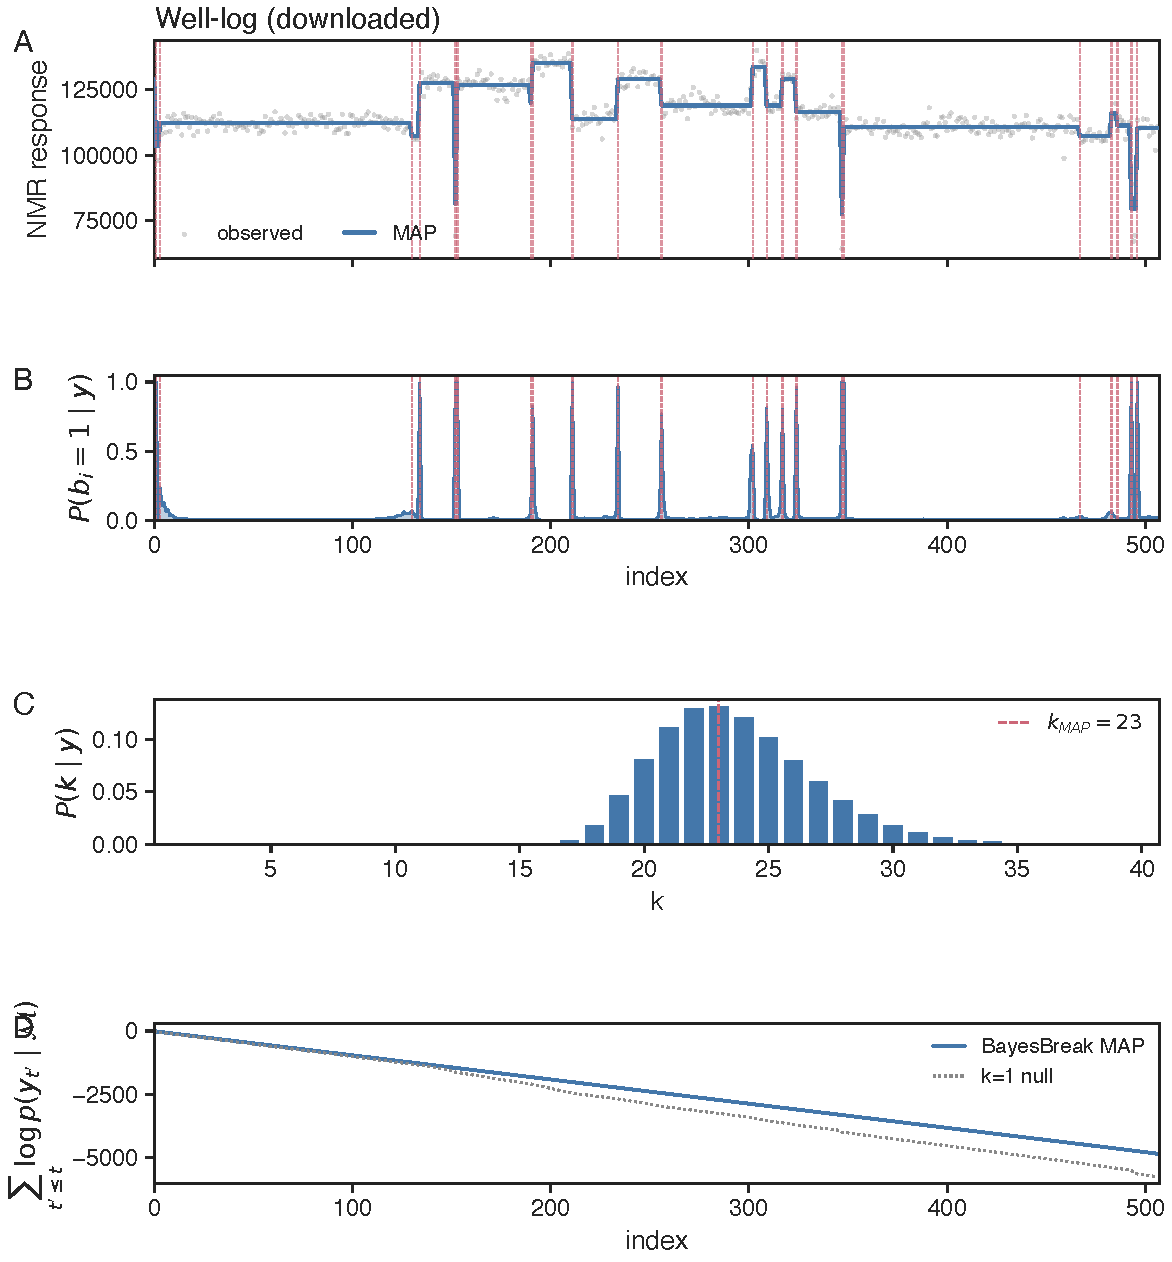
\includegraphics[width=0.95\textwidth]{shared/figures/results/fig6_welllog.pdf}
  \caption{Executed well-log fit. Solid segmentation and red markers are fitted summaries; boundary probabilities and $p(k\mid y)$ are posterior quantities; the cumulative panel is in-sample.}
  \label{fig:welllog-paper}
\end{figure*}

\paragraph{Array-CGH.}
The shared-boundary model used 43 subjects on 2,215 probes, selected the maximum considered 15 segments, and recorded pooled log evidence $76359.79958695151$ (Figure~\ref{fig:cgh-paper}). The sum of independently fitted subject evidences was $109617.69544504143$, but the two totals arise from different factorizations and are not a direct Bayes factor.

\begin{figure*}[t]
  \centering
  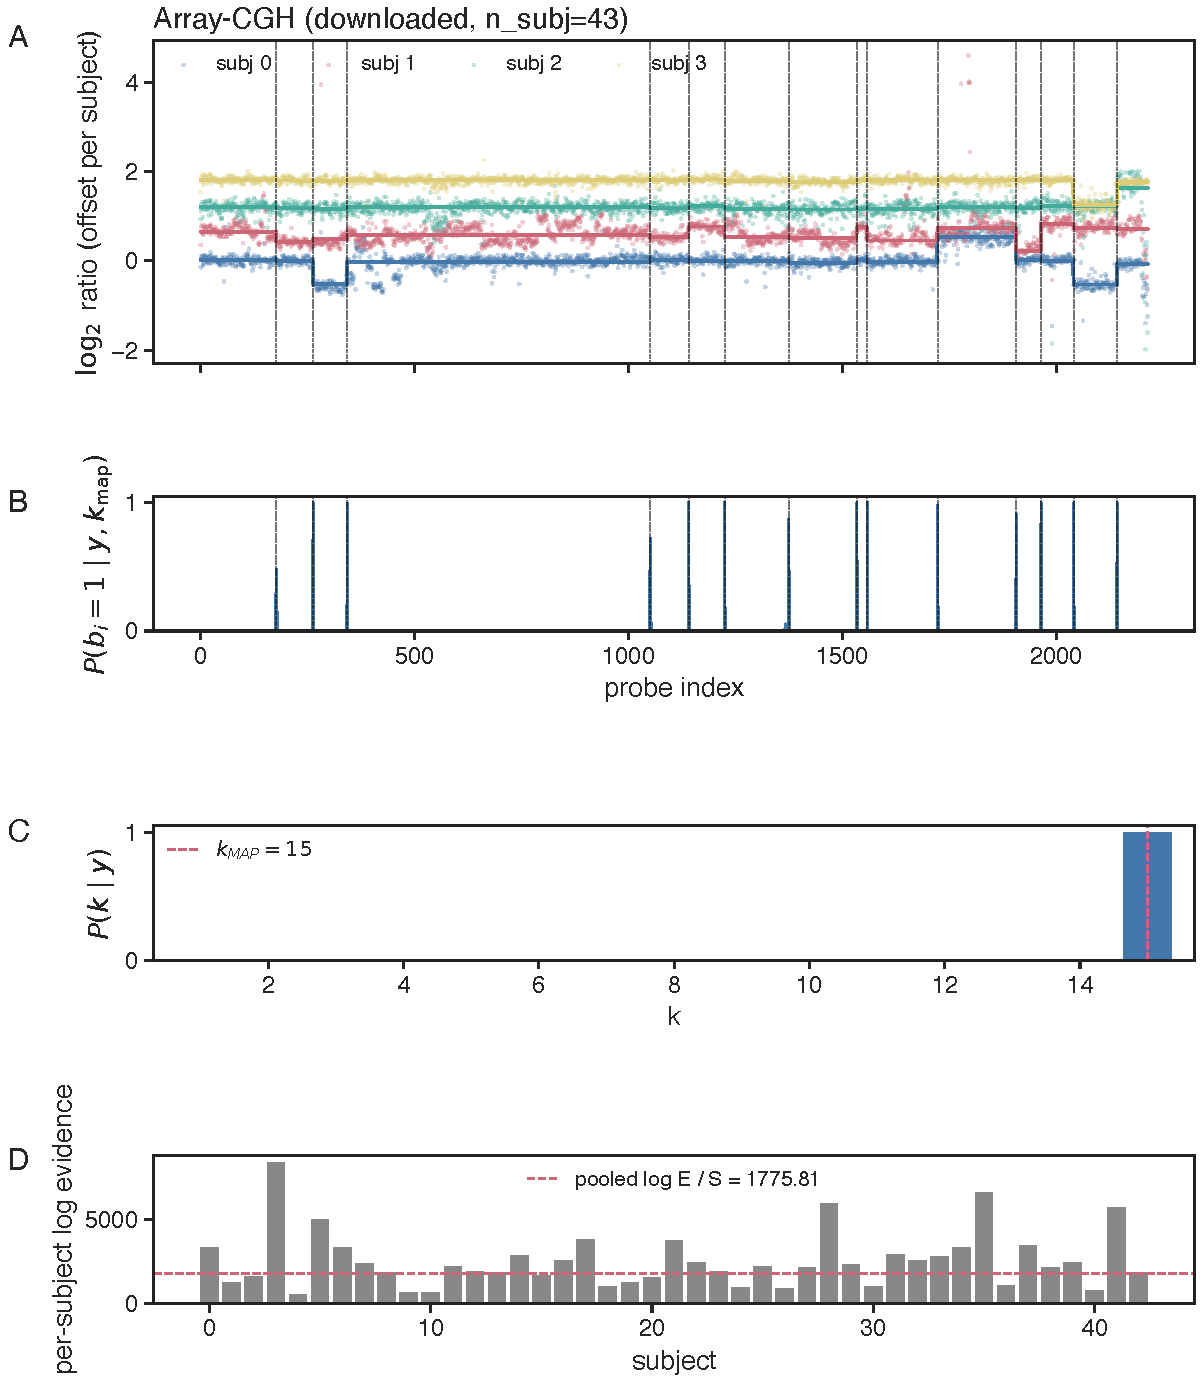
\includegraphics[width=0.95\textwidth]{shared/figures/results/fig7_cgh.pdf}
  \caption{Executed shared-boundary array-CGH fit. The common red markers are fitted joint-MAP boundaries, not external copy-number annotations.}
  \label{fig:cgh-paper}
\end{figure*}

\begin{exclusionbox}[\resultid{RES-BB-CMP-002}: incompatible comparator axis]
The comparator cache flattened a $43\times2215$ fitted matrix to 95,245 values while retaining reference boundaries on the 2,215-probe axis. Its zero agreement scores are real executions of an incompatible comparison and are excluded from scientific comparison. The corrected child below uses the raw subject-by-probe matrix, validated probe coordinates, and a new result identifier.
\end{exclusionbox}

The corrected child \resultid{RES-BB-CMP-003} used the exact hashed raw $2{,}215\times43$ probe-by-subject matrix and scored every method on the common probe-index axis (Figure~\ref{fig:cgh-agreement-corrected-paper}). Agreement $F_1@3$ with the model-derived BayesBreak MAP was $0.8000$ for PELT, $0.9286$ for dynamic programming, $0.7143$ for binary segmentation, and $0.7857$ for wild binary segmentation. Dynamic programming, binary segmentation, and wild binary segmentation used the 14-boundary target. The predeclared eight-value PELT grid did not attain 14 boundaries; its closest candidate returned 11 and was not retuned post hoc. These are agreement diagnostics, not external biological accuracy or predictive superiority.

\begin{figure*}[t]
  \centering
  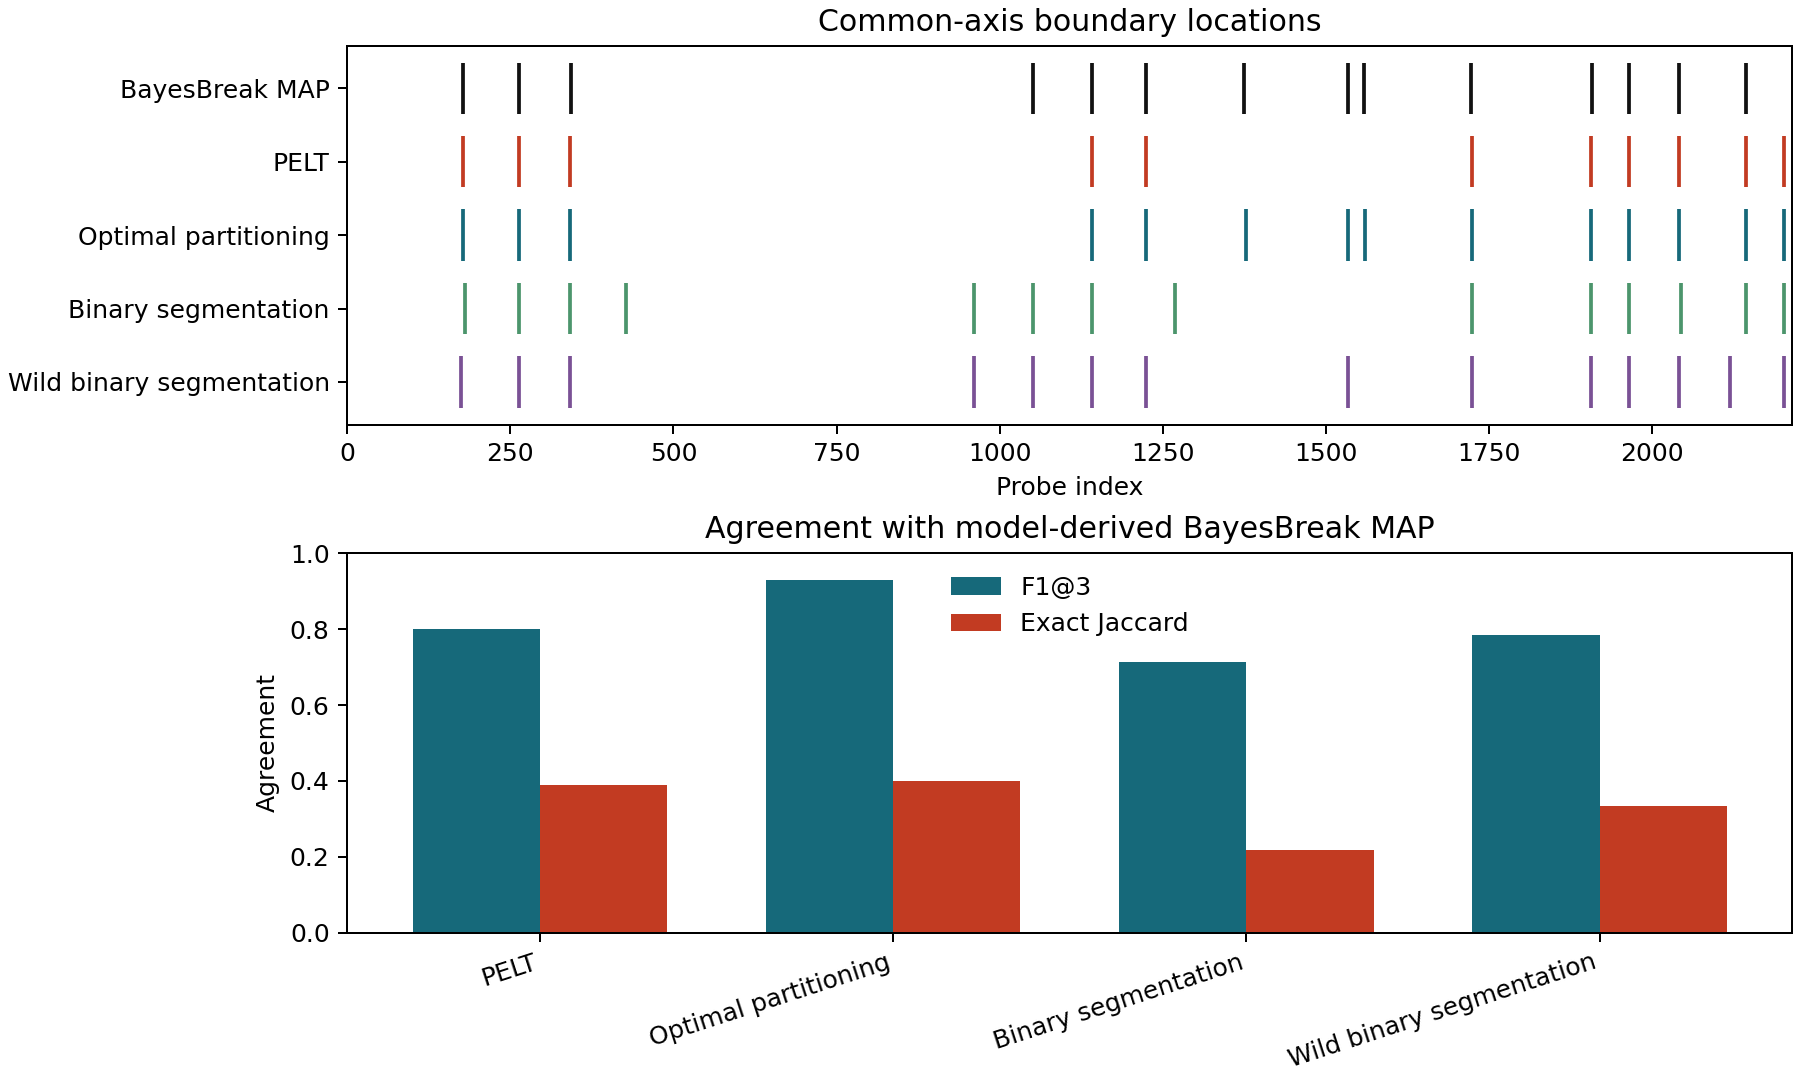
\includegraphics[width=0.94\textwidth]{shared/figures/results/fig_phase6_cgh_agreement.png}
  \caption{Corrected common-axis array-CGH comparison \resultid{RES-BB-CMP-003}. Top: boundary locations on the shared probe axis. Bottom: $F_1@3$ and exact Jaccard agreement with the model-derived BayesBreak MAP.}
  \label{fig:cgh-agreement-corrected-paper}
\end{figure*}

\paragraph{S\&P 500 volatility.}
The source covers January 1, 2015 through December 31, 2023, with approximately 2,263 raw observations and an executed stride-four series of $n=566$. The Gaussian log-squared-return model selected 29 segments with log evidence $-1296.6537252802884$ (Figure~\ref{fig:spx-paper}). A secondary Bernoulli threshold-incidence signal selected 50 segments with log evidence $-114.41004640965144$. It is a different response model, not a Poisson count, and its evidence is not directly comparable with the Gaussian total.

\begin{figure*}[t]
  \centering
  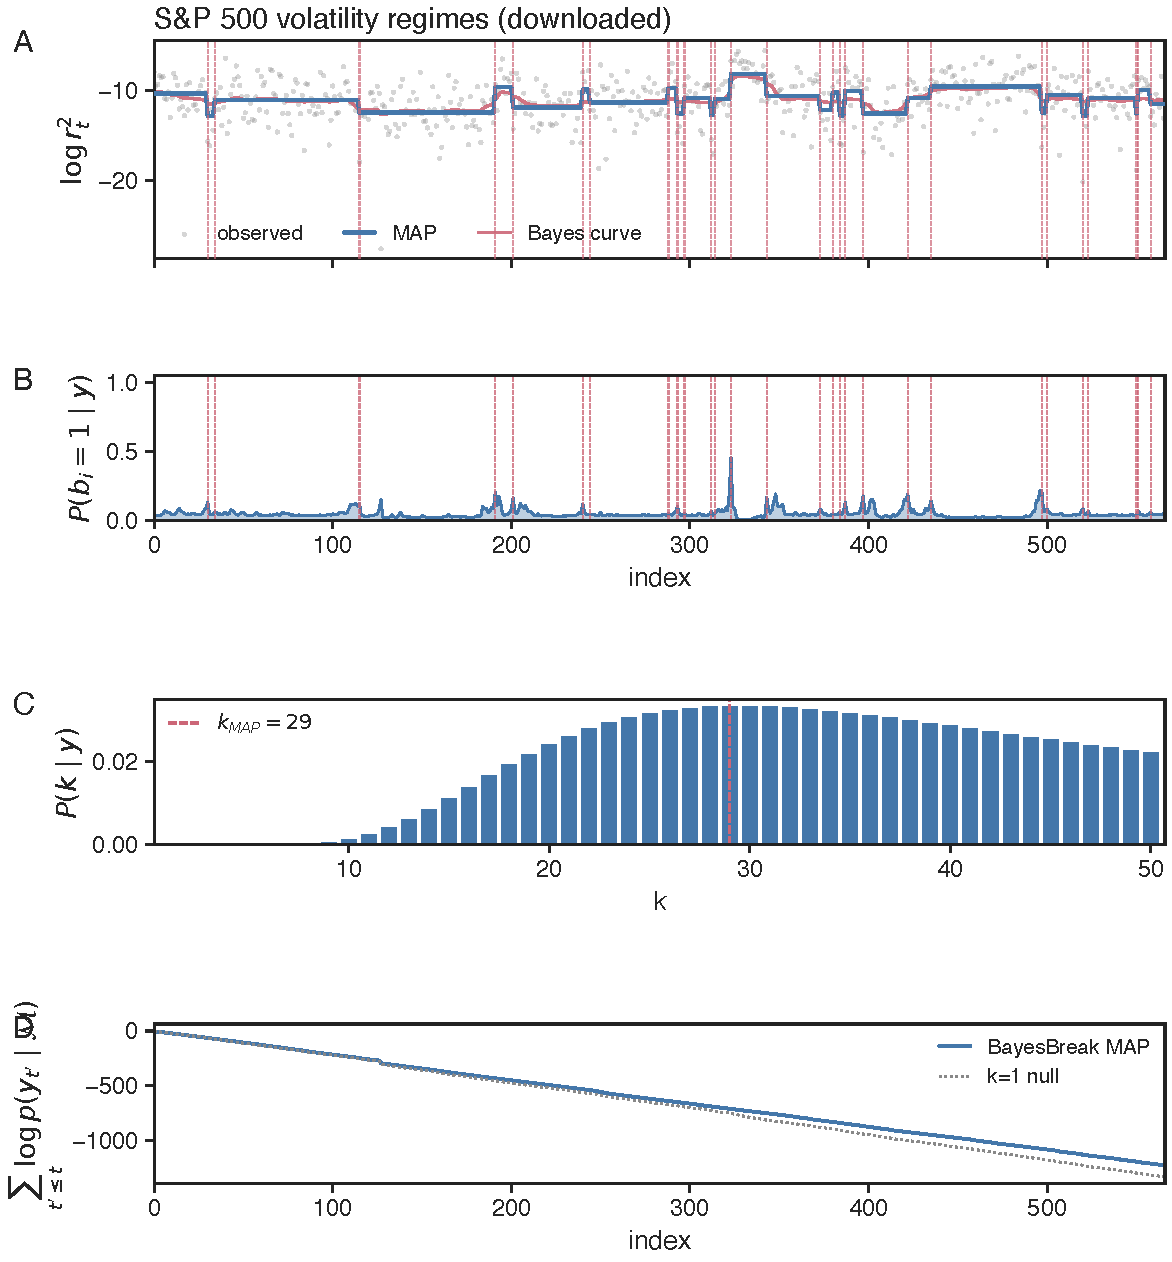
\includegraphics[width=0.95\textwidth]{shared/figures/results/fig8_spx.pdf}
  \caption{Executed S\&P 500 volatility fit after archived stride-four preprocessing. Red markers are fitted boundaries, not independently annotated macroeconomic events.}
  \label{fig:spx-paper}
\end{figure*}

\paragraph{Methylation.}
The executed data are the \texttt{methylKit} \texttt{test1.myCpG} chromosome-21 example with 1,904 CpGs and per-CpG read coverage used as known precision. The Beta-valued quadrature model selected 15 segments and recorded log evidence $-9518.667508691196$ (Figure~\ref{fig:methylation-paper}). This is not the previously described methylation-atlas analysis. The segmentation fit remains admissible descriptive evidence; the archived held-out value is excluded from predictive conclusions under Definition~\ref{def:heldout-score-paper}.

\begin{figure*}[t]
  \centering
  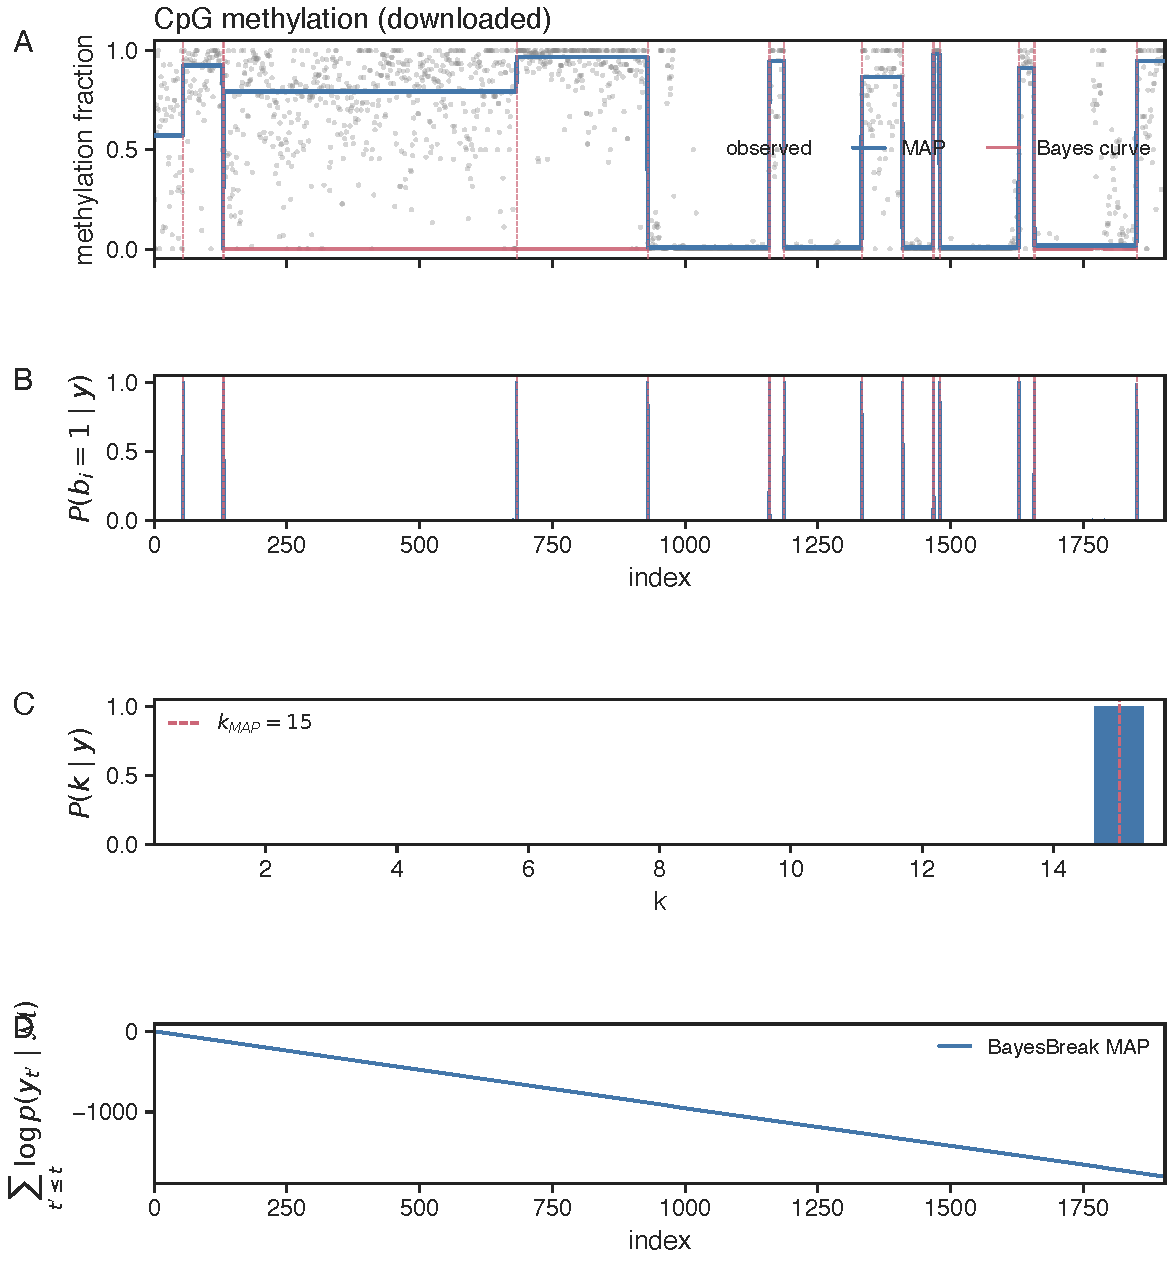
\includegraphics[width=0.95\textwidth]{shared/figures/results/fig9_methylation.pdf}
  \caption{Executed Beta-valued fit to the methylKit chromosome-21 example. Red markers are fitted MAP boundaries; no independent atlas transition annotation was archived.}
  \label{fig:methylation-paper}
\end{figure*}

\begin{exclusionbox}[\resultid{RES-BB-RD-007Q}: invalid family/support predictive path]
The archived held-out value $-387.50040013308154$ for $m=381$ remains historical provenance. It used a Gaussian predictive fallback for a Beta-observation estimator and assigned coordinates beyond fitted support to the endpoint block, so it remains excluded from posterior-predictive conclusions.
\end{exclusionbox}

The corrected child \resultid{RES-BB-RD-008Q} used the Beta-observation predictive distribution, observed held-out coverage as positive $\phi_{\mathrm{new}}$, and \texttt{extrapolation=error}. Ten disjoint stratified interior blocks held out 1,520 CpGs while retaining both fitted-support endpoints. Total log predictive score was $-23605.6749$ and pooled mean score was $-15.5300$; the mean split score had a 95\% $t$ interval $[-23.1445,-7.9156]$. Mean boundary-stability $F_1@3$ against the model-derived full-data MAP was $0.8786$ (Figure~\ref{fig:methyl-predictive-corrected-paper}). The blocks are regions of one chromosome rather than independent biological samples, and no certified Beta-observation PIT or external atlas accuracy is reported. Because both family and split changed, this score is not numerically comparable with the excluded parent.

\begin{figure*}[t]
  \centering
  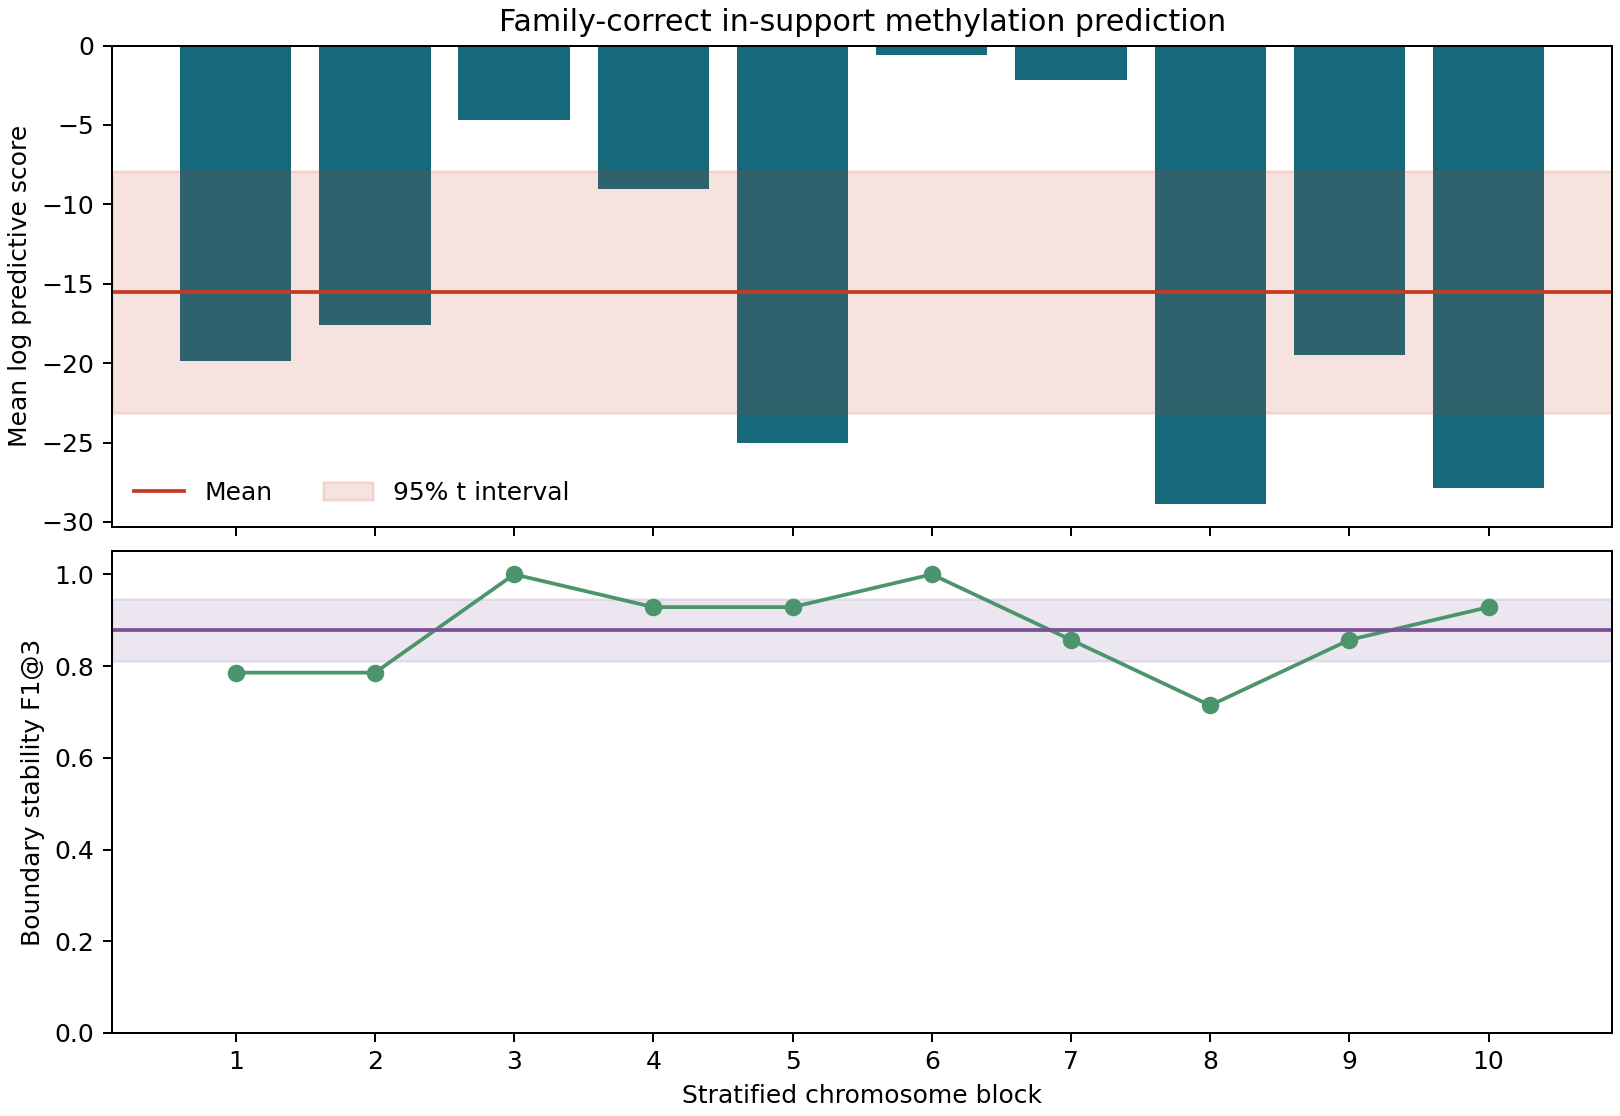
\includegraphics[width=0.88\textwidth]{shared/figures/results/fig_phase6_methyl_predictive.png}
  \caption{Corrected methylation posterior prediction \resultid{RES-BB-RD-008Q}. Top: mean Beta-observation log predictive score across ten in-support chromosome blocks. Bottom: boundary-stability $F_1@3$ against the model-derived full-data MAP. Shaded bands are split-level 95\% $t$ intervals.}
  \label{fig:methyl-predictive-corrected-paper}
\end{figure*}

\subsection{What the executed record establishes}
The executed record demonstrates that common partition recursions can use closed-form conjugate segment marginal likelihoods, one-dimensional quadrature, other numerical segment calculations, shared-changepoint pooling, and finite latent-group templates. It provides calibrated boundary probabilities in one Gaussian simulation design, a corrected finite latent-group stress grid, finite-range runtime measurements, four traceable real-data fits, a corrected common-axis CGH agreement diagnostic, and a corrected family-specific methylation predictive evaluation. It does not yet establish external boundary accuracy, dominance under independently tuned predictive comparisons, robustness across broad misspecification regimes, routine-wide approximation guarantees, or asymptotic speed better than the quadratic dynamic-programming bound.
